\documentclass[11pt]{article}

%\pagestyle{headings}

\textwidth=440pt
\hoffset=-0.6truein

\usepackage{amsmath}
\usepackage{amsfonts}
\usepackage{amssymb}
\usepackage{authblk}
\usepackage{dsfont}
\usepackage{pifont}
\usepackage{booktabs}
\usepackage{tabularx}
\usepackage{siunitx}
%\usepackage{bbold}
\usepackage{graphicx}
\usepackage{epstopdf}
\usepackage{epsfig}
%\usepackage{bibunits}
%\usepackage{theorem}
%\usepackage[framed]{ntheorem}
\usepackage{framed}
%\usepackage{showlabels}
\usepackage{makeidx}
\usepackage{simplewick}
%\usepackage{tikz-feynman}
\usepackage{hyperref}
\usepackage{placeins}
\usepackage{bbold}
\usepackage[font=small,labelfont=bf]{caption}
%\tikzfeynmanset{compat=1.0.0}
\usepackage{tikz}
\usepackage{braket}
\usetikzlibrary{positioning}% To get more advances positioning options
\usetikzlibrary{arrows}
\usetikzlibrary{colorbrewer}

% barn deprecated by siunitx
\DeclareSIUnit{\barn}{b}

% General global commands
%\newcommand{\cov}{C}
\newcommand{\posterior}[1]{\tilde{#1}}
\newcommand{\real}{\mathbb{R}}
\newcommand{\textin}{\text{in}} 

% General inverse Problems
% map operators
\newcommand{\fwdmapop}{G}
\newcommand{\obsop}{O}
\newcommand{\fwdobsop}{\mathcal{\fwdmapop}}
% model space
\newcommand{\nmodel}{N_{\rm model}}
\newcommand{\modelspace}{X}
\newcommand{\modelvec}{u}
\newcommand{\modelpriorcent}{\modelvec_0}
\newcommand{\modelpriorcov}{\cov_X}
\newcommand{\modelpostcent}{\posterior{\modelvec}}
\newcommand{\modelpostcov}{\posterior{\cov}_X}
% observable space
\newcommand{\ndata}{N_{\rm data}}
\newcommand{\obs}{y}
\newcommand{\obspriorcent}{\obs_0}
\newcommand{\obspriorcov}{\cov_{Y}}
\newcommand{\obsnoise}{\eta}
\newcommand{\obspostcent}{\posterior{\obs}}
\newcommand{\obspostcov}{\posterior{\cov}_Y}
% linear map
\newcommand{\linmap}{\fwdobsop}
\newcommand{\vander}{\mathcal{X}}
\newcommand{\nlaw}{N_{\rm law}}

% NNPDF data/model
\newcommand{\law}{f}
\newcommand{\pseudodat}{\mu}
\newcommand{\noise}{\epsilon}
\newcommand{\repind}{(k)}
\newcommand{\modelvecrep}{\modelvec_*^{\repind}}
% likelihood
\newcommand{\likelihood}{\mathcal{L}}
\newcommand{\repchis}{{\chi^2}^{\repind}}

% closure fitting
\newcommand{\lawmodel}{w}
\newcommand{\utrue}{u_\mathrm{true}}
\newcommand{\uest}{u_\mathrm{est}}

% closure estimators
\newcommand{\testset}[1]{ {{#1}^{\prime}} }
\newcommand{\emodel}[1]{ \mathbf{E}_{\{ \modelvec_* \}} \left[ #1 \right] }
\newcommand{\eout}{\mathcal{E}^{\rm out}}

\newcommand{\nfits}{N_{\rm fits}}
\newcommand{\nreps}{N_{\rm rep}}

\newcommand{\bias}{{\rm bias}}
\newcommand{\var}{{\rm variance}}
\newcommand{\covrep}{\testset{\cov}^{(\rm replica)}}
\newcommand{\covcent}{\testset{\cov}^{(\rm central)}}
\newcommand{\biasvarratio}{\mathcal{R}_{bv}}

% quantile estimators
\newcommand{\xisigdat}[1]{\xi^{(\rm data)}_{#1 \testset{\sigma}}}
\newcommand{\xisigdati}[1]{\xi^{(\rm data)}_{#1 {\testset{\sigma}_i}}}
\newcommand{\modelstd}{\hat{\sigma}}
\newcommand{\erf}{{\rm erf}}

% abbreviations
\newcommand{\ie}{{\it i.e.}}
\newcommand{\eg}{{\it e.g.}}
\newcommand{\viz}{{\it viz.}}

% delta chi2 appendix
\newcommand{\ein}{\mathcal{E}^{\rm in}}
\newcommand{\deltachi}{\Delta_{\chi^2}}
\newcommand{\noisecross}{{\rm noise \, cross \, term}}

% -------------------%
% deprecated commands
% -------------------%
\newcommand{\vv}[1]{\mathbf{#1}}

\newcommand{\vecdiffreptwo}{\left( \vv{\model}^{\repind} - \vv{\levtwo}^{\repind}  \right)}
\newcommand{\vecdiffcentone}{\left( \erep{\vv{\model}} - \vv{\levone} \right)}

\newcommand{\coveig}{\sigma^{2}}
\newcommand{\diag}[1]{\hat{#1}}

\newcommand{\levelonediff}{\Delta}
\newcommand{\underlyingdiff}{u}
\newcommand{\repdiff}{v}

\newcommand{\shiftcross}{{\rm shift \, cross \, term}}
\newcommand{\deltaeps}{\Delta_{\epsilon}}
\newcommand{\kldiv}{D_{KL}}

\newcommand{\diffreptwo}{\left( \model^{\repind} - \levtwo^{\repind} \right)}
\newcommand{\diffcentone}{\left( \erep{\model} - \levone \right)}
\newcommand{\diffcentunder}{\left( \erep{\model} - \law \right)}
\newcommand{\diffcentrep}{\left( \erep{\model} - \model^{\repind}\right)}

\newcommand{\invcov}[1]{\cov^{-1}_{#1}}
\newcommand{\erep}[1]{\mathbf{E}_{\noise}\left[ #1 \right]}
\newcommand{\eshift}[1]{\mathbf{E}_{\shift}\left[ #1 \right]}

\newcommand{\model}{\fwdobsop}
\newcommand{\shift}{\obsnoise}
\newcommand{\invcovprime}{C_D^{\prime -1}}
\newcommand{\levone}{z}
\newcommand{\levtwo}{y}

\newcommand{\npoints}{N_{\rm points}}
\newcommand{\nfit}{\texttt{n3fit}}

\newcommand{\ndat}{N_{\mathrm{dat}}}
\newcommand{\ngrid}{N_{\mathrm{grid}}}
\newcommand{\nflav}{N_{f}}
\newcommand{\NThetaPar}{N_{\Theta\parallel}}
\newcommand{\NThetaPerp}{N_{\Theta\perp}}   
%\newcommand{\nmodel}{N_{\mathrm{model}}}
\newcommand{\cov}{\mathrm{Cov}}
\newcommand{\FKtab}{(\mathrm{FK})}
\newcommand{\FKtabT}{(\mathrm{FK})^T}
\newcommand{\GP}{\mathcal{GP}}
\newcommand{\lat}{{\mathrm{lat}}}
\newcommand{\lin}{{\mathrm{lin}}}
\newcommand{\PDF}{\textrm{PDF}}
\newcommand{\B}{\mathcal{B}} % Basis
\newcommand{\RPDF}{\mathbb{R}^{\PDF}}
\newcommand{\RRPDF}{\mathbb{R}^{\PDF \times \PDF}}
\newcommand{\ddt}{\frac{d}{dt}}
\newcommand{\fin}{f^{\rm in}}

% Matrix
\newcommand{\bpmat}{\begin{pmatrix}}
\newcommand{\epmat}{\end{pmatrix}}

\graphicspath{{./figs/}}

\title{Notes on Neural Tangent Kernels}
\author[b]{Luigi Del Debbio} 
\affil[b]{Higgs Centre for Theoretical Physics, School of Physics and Astronomy,
Peter~Guthrie~Tait~Road, Edinburgh EH9 3 FD, United Kingdom.}

\date{\today}
\makeindex

\begin{document}

\maketitle

\begin{abstract}
    Summary of results for NTKs. These notes follow the notation 
    introduced in Ref.~\cite{DBLP:journals/corr/abs-1806-07572}.
\end{abstract}

\section{Definitions}
\label{sec:defs}

\subsection{Neural Networks}
\label{sec:NNDef}

We consider the case of neural networks (NNs) with $L+1$ layers, labelled by the
index $\ell=0,\ldots,L$. The number of neurons in layer $\ell$ is denoted by
$n_{\ell}$. The $\ell=0$ and $\ell=L$ layers are the input and output layers
respectively, so that a NN parametrizes an element of 
\begin{align}
    \label{eq:SetF}
    \mathcal{F} = \left\{ 
        f: \mathbb{R}^{n_0} \to \mathbb{R}^{n_L}
    \right\}\, .
\end{align}
The space of inputs in this case is $\mathcal{X}=\mathbb{R}^{n_0}$, while the
space of outputs is $\mathcal{Y}=\mathbb{R}^{n_L}$. The number of parameters
used in the parametrization is the total number of weights and biases,
\begin{align}
    \label{eq:NumOfPars}
    P = \sum_{\ell=0}^{L-1} (n_\ell + 1) n_{\ell+1}\, .
\end{align}
The weights connecting the layer $\ell$ to the layer $\ell+1$ are denoted
$W^{(\ell+1)}$ and the biases in layer $\ell+1$ are denoted $b^{(\ell+1)}$. 
With this convention
\begin{align}
    W^{(\ell+1)} \in \mathbb{R}^{n_{\ell+1}\times n_{\ell}}\, ,
    \quad 
    b^{(\ell+1)} \in \mathbb{R}^{\ell+1}\, .
\end{align}
When referring to the whole set of parameters, we use the symbol 
\begin{align}
    \theta = \left\{
        W^{(\ell)}, b^{(\ell)}; \; \ell=0, \ldots, L-1
    \right\}\, , 
\end{align}
while individual parameters are denoted $\theta_\mu$, with $\mu=1, \ldots, P$.

The input space is
$\mathcal{X}=\mathbb{R}^{n_0}$ and we consider a probability distribution
$p^{\textin}$ over $\mathcal{X}$, which induces a scalar product in
$\mathcal{F}$,
\begin{align}
    \label{eq:ScalProdX}
    \langle f, g\rangle_{\textin} &= 
        \mathbb{E}_{x\sim p^{\textin}} \left[f(x)^T g(x)\right] \\
        &= \int dx\, p^{\textin}(x) f_i(x) g_i(x)\, .
\end{align}
For a discrete set of datapoints $\mathcal{D}$, 
\begin{align}
    p^{\textin}(x) = \frac{1}{|\mathcal{D}|} \sum_{\alpha\in\mathcal{D}} 
        \delta(x-x_{\alpha})\, ,
\end{align}
where the index $\alpha$ labels the elements of the dataset. For a given set of
parameters, the function parametrized by the NN, which we denote $f_{\theta}$, is given by the
preactivation function of the output layer $L$,
\begin{align}
    f(x;\theta) = \phi^{(L)}(x)\, .
\end{align}
The preactivations $\phi^{(\ell)}$ and the activations $\rho^{(\ell)}$ are
defined recursively as
\begin{align}
    \rho^{(0)}_i(x) 
        &= x_i\, , \\
    \phi^{(\ell+1)}_i(x)
        &= \sum_{j=1}^{n_\ell} W^{(\ell+1)}_{ij} \rho^{(\ell)}_j(x) + b^{(\ell+1)}_i\, , \\
    \rho^{(\ell)}_i(x)
        &= \rho\bigl(\phi^{\ell}_i(x)\bigr)\, ,
\end{align}
where $\rho$ is the activation function. The function 
\begin{align}
    F^{(L)} 
        :\quad & \mathbb{R}^P \to \mathcal{F} \\
        & \theta \mapsto F^{(L)}(\theta) = f_{\theta}
\end{align}
is called the NN realization function. We also introduce the (dual) space of
linear functionals acting on $\mathcal{F }$,
\begin{align}
    \label{eq:FdualDef}
    \mathcal{F}^* = 
        \left\{
            \mu: \mathcal{F} \to \mathbb{R}\,; \; 
                \mu = \langle d, \cdot\rangle_{\textin}, \; d \in \mathcal{F}
        \right\}\, ,
\end{align}
and a loss function 
\begin{align}
    \label{eq:LossDef}
    \mathcal{L}\, : \mathcal{F}\times \mathcal{Z} \to \mathbb{R}\, .
\end{align}
Here $\mathcal{Z}$ denotes the space of datapoints, which we can identify for
now with $\mathcal{X}\times\mathcal{Y}$. 

% The cost function for a set of
% datapoints $\mathcal{D}$ is defined as 
% \begin{align}
%     \label{eq:CostDef}
%     C_{\mathcal{D}}(f) = \frac{1}{|\mathcal{D}|} \sum_{\alpha\in\mathcal{D}}
%     \mathcal{L}(f,z_{\alpha})\, .
% \end{align}

\subsection{Kernel Gradient}
\label{sec:KernGradDef}

A kernel $K$ is defined as a symmetric function 
\begin{align}
    \label{eq:KernDef}
    K: \mathbb{R}^{n_0} \times \mathbb{R}^{n_0} \to 
    \mathbb{R}^{n_L\times n_L}\, ,
\end{align}
such that $K(x,x')=K(x',x)^T$. Using the kernel, a bilinear map is defined 
on $\mathcal{F}$
\begin{align}
    \label{eq:KMap}
    \langle f,g\rangle_K = \mathbb{E}_{x,x'\sim p^{\textin}}
    \left[
        f(x)^T K(x,x') g(x')
    \right]\, .
\end{align}
The kernel is positive definite if
\begin{align}
    ||f||_{p^{\textin}} > 0 
    \quad \Longrightarrow \quad
    ||f||_K > 0\, .
\end{align}
Given a kernel $K$, we define a map
\begin{align}
    \label{eq:PhiKMap}
    \Phi_K: \mathcal{F}^* &\to \mathcal{F} \\
            \mu &\mapsto f_{\mu}\, ,
\end{align}
such that 
\begin{align}
    f_{\mu,i}(x) 
        &= \langle d, K_{i\cdot}(x,\cdot) \rangle_{p^{\textin}} \\
        &= \sum_{j=1}^{n_L} \int dx'\, p^{\textin}(x')\, d_j(x')
            K_{ij}(x,x')\, ,
\end{align}
where $d\in\mathcal{F}$, and $\mu=\langle d, \cdot\rangle_{p^{\textin}}$.

The cost function for a given dataset depends on the values of the function 
$f$ at the datapoints $x_{\alpha}$, so that we can write
\begin{align}
    C_{\mathcal{D}}(f) = \widehat{C}(\mathbf{f})\, ,
\end{align}
where $\mathbf{f}$ is the finite-dimensional vector made of the 
values $f_{\alpha}=f(x_{\alpha})$ for $\alpha=1, \ldots, |\mathcal{D}|$.
The variation of the cost function at a point $f_0 \in \mathcal{F}$ is
\begin{align}
    \left. \delta C_{\mathcal{D}} \right|_{f_0} 
        &= C_{\mathcal{D}}(f_0+\delta f) - C_{\mathcal{D}}(f_0) \\
        &= \sum_{\alpha\in\mathcal{D}} 
            \left. \frac{\partial \widehat{C}}{\partial f_\alpha} \right|_{f_0} 
            \delta f_{\alpha} \\
        &= \left. \partial^{\textin}_{f} C \right|_{f_0} \delta f \\
        &= \langle \left. d\right|_{f_0}, \delta f\rangle_{p^{\textin}}\, ,
\end{align}
where $\delta f \in \mathcal{F}$, $\delta f_{\alpha}=\delta f(x_{\alpha})$ and 
$\displaystyle \left. \partial^{\textin}_{f} C \right|_{f_0} \in \mathcal{F}^*$.

Using the kernel $K$, the {\em kernel gradient} $\left.\nabla_K C\right|_{f_0}$
is defined as 
$\displaystyle \Phi_K\left(\left. \partial^{\textin}_{f} C \right|_{f_0}
\right)$, \ie 
\begin{align}
    \label{eq:KernGradC}
    \left.\nabla_K C\right|_{f_0}(x)
        &= \frac{1}{|\mathcal{D}|} \sum_{\alpha\in\mathcal{D}} 
            K(x,x_{\alpha}) \left. 
            \frac{\partial \widehat{C}}{\partial f_\alpha}\right|_{f_0}\, .
\end{align}
A function $f(t)$ follows the kernel gradient descent if 
\begin{align}
    \partial_{t} f(t) = -\left.\nabla_{K} C\right|_{f(t)}\,.
\end{align}
During the kernel descent, the cost function variation is given by
\begin{align}
    \partial_{t} \left. C\right|_{f(t)}
        &= - \langle \left. d \right|_{f(t)}, \left.\nabla_{K} C\right|_{f(t)} \rangle_{p^{\textin}} = 
        -|| \left. d \right|_{f(t)} ||^2_{K}\, .
\end{align}
More generally, for a function $\widehat{O}$ that depends on 
the values of $f$ on the points in the dataset, 
\begin{align}
    \partial_{t} \left. \widehat{O}\right|_{f(t)}
        &= - \left\langle 
            \frac{\partial \widehat{O}}{\partial f}, 
            \frac{\partial \widehat{C}}{\partial f} 
            \right\rangle_K\, .
\end{align}

\section{Gradient Descent for NNPDF}
\label{sec:GradDescNNPDF}

We work in a basis where the data covariance $C_Y$ is diagonal. Such a choice has two main advantages:
\begin{enumerate}
    \item The data points in this basis are statistically independent, so that when the data is split, 
    e.g. between training and validation sets, the points in each subset are not correlated. 
    \item Working in a basis where the data covariance is diagonal, requires to compute the eigenvectors
    and eigenvalues of $C_Y$, thereby automatically checking for a potentially large condition number. 
\end{enumerate}
Note that, in case we need to apply kinematic cuts, these can be applied before rotating to the diagonal basis. The diagonal basis is then defined by determining the eigensystem of the reduced covariance matrix, i.e. the matrix obtained by removing the lines and columns that correspond to data points that do not pass the kinematic cuts.  

The loss function is defined to be the Mean Square Error (MSE),
\begin{align}
    \label{eq:MSELoss}
    \mathcal{L} &= \frac12 \left(y - T\right)^T C_Y^{-1} \left(y - T\right)\, , \\
        &= \frac12 ||y-T||^2_{C_Y}\, ,
\end{align}
where 
\begin{align}
    \label{eq:DataAndTheory}
    y = 
        \begin{pmatrix}
            y_1 \\
            \vdots \\
            y_I \\
            \vdots \\
            y_{\ndat}
        \end{pmatrix}\, , 
    \quad \mathrm{and} \quad 
    T = 
        \begin{pmatrix}
            T_1 \\
            \vdots \\
            T_I \\
            \vdots \\
            T_{\ndat}
        \end{pmatrix}\, 
\end{align}
are vectors containing the data points $y_I$ and their respective theoretical predictions $T_I$, where $I=1, \dots, \ndat$. The loss function can be written using explicit indices, 
\begin{align}
    \label{eq:MSELossWithIndices}
    \mathcal{L} = \frac12 \sum_I \frac{1}{\sigma_I^2} \left(y_I - T_I\right)^2\, .
\end{align}
However, here and in what follows, we try to minimize the usage of explicit indices.

Denoting by $t$ the training time, and by $\theta_\mu$, with $\mu=1, \dots, P$, the parameters used to specify 
the functional form of $f$, gradient descent is defined by the flow equation, 
\begin{align}
    \label{eq:GradD}
    \frac{d}{dt} \theta_{\mu,t} = - \sum_{\nu} \lambda_{\mu\nu} \nabla_\nu \mathcal{L}_t\, , 
\end{align}
where we added a suffix $\mathcal{L}_t$ to emphasise that the loss function is evaluated using the function $f_t$ at training time $t$. 
We introduced the tensor $\lambda_{\mu\nu}$ to take into account the case of a non-trivial metric in the space of parameters. We will use $\lambda_{\mu\nu} = \lambda_{\mu} \delta_{\mu\nu}$, 
unless explicitly stated.
The gradient on the RHS of Eq.~\ref{eq:GradD} above is
\begin{align}
    \label{eq:GradStepOne}
    \nabla_\mu \mathcal{L}_t = 
        - \left(\nabla_\mu f_t\right)^T \left(\frac{\partial T}{\partial f}\right)_t^T 
        C_Y^{-1} \epsilon_t\, ,
\end{align}
where we introduced $\epsilon_t=y-T_t$, to denote the difference between the data and the theoretical prediction obtained from $f_t$. 
The quantities that depend on the training time have an explicit suffix $t$. Using the chain rule yields
\begin{align}
    \frac{d}{dt} f_t 
        \label{eq:NtkOne}
        &=  \sum_{\mu}\, \left(\nabla_{\mu} f_t\right) \, \frac{d}{dt} \theta_{\mu,t} \\
        \label{eq:NtkTwo}
        &=  \left[\sum_{\mu,\nu}\, \lambda_{\mu\nu} \left(\nabla_\mu f_t\right)\, 
                    \left(\nabla_\nu f_t\right)^T\right]\,  
                \left(\frac{\partial T}{\partial f}\right)_t^T C_Y^{-1} \epsilon_t\, .
\end{align}
Introducing the Neural Tangent Kernel (NTK), 
\begin{align}
    \label{eq:NTKDefNoIndices}
    \Theta_t = \sum_{\mu,\nu}\, \lambda_{\mu\nu} \left(\nabla_\mu f_t\right)\, 
        \left(\nabla_\nu f_t\right)^T\, ,
\end{align}
or equivalently using explicit indices for once,
\begin{align}
    \label{eq:NTKDef}
    \Theta_{\delta_1\delta_2,t} = \sum_{\mu\nu} \lambda_{\mu\nu} \nabla_\mu f_{\delta_1,t}\, \nabla_\nu f_{\delta_2,t}\, .
\end{align}
Note that the NTK is a tensor in the space of the grid points on which the function $f$ is evaluated, \ie \
$f_{\delta} = f(x_\delta)$.

The flow equation becomes
\begin{align}
    \label{eq:FlowWithNTKNoIndices}
    \frac{d}{dt} f_t = 
        \Theta_t \left(\frac{\partial T}{\partial f}\right)_t^T C_Y^{-1} \epsilon_t\, .
\end{align}
This flow equation is completely general, for any parametrization and any dependence of the theoretical predictions on the function f.

Let us now focus on the case where the theoretical prediction is linear in $f$, 
\begin{align}
    \label{eq:LinearDataFK}
    T_I = \FKtab_{I\alpha} f_\alpha\, ,
\end{align}
so that 
\begin{align}
    \label{eq:LinearNabla}
    \left(\frac{\partial T_I}{\partial f_\alpha}\right) = \FKtab_{I\alpha}\, ,
\end{align}
is actually independent of $t$. Note in passing that $\FKtab$ is not a square matrix, and hence not invertible. 

The loss function is a quadratic form in $f$,
\begin{align}
    \label{eq:QuadraticLossInf}
    2 \mathcal{L} = f^T M f - f^T \FKtabT C_Y^{-1} y - y^T C_Y^{-1} \FKtab f + y^T C_Y^{-1} y \, .
\end{align}
We can restrict $f$ to the subspace orthogonal to $\ker\FKtab$; the components in $\ker\FKtab$ do not 
enter the loss function and therefore are unconstrained. In this subspace, the matrix 
\begin{align}
    \label{eq:MmatrixForLoss}
    M = \FKtabT C_Y^{-1} \FKtab
\end{align}
is symmetric and positive definite, and hence invertible. Rewriting 
\begin{align}
    \label{eq:CompleteTheSquare}
    f = \chi + M^{-1} \FKtabT C_Y^{-1} y\, ,
\end{align}
yields
\begin{align}
    \label{eq:LossFunctionOfChi}
    2 \mathcal{L} = \chi^T M \chi +
        y^T C_Y^{-1} \left[
            1 - \FKtab M^{-1} \FKtabT C_Y^{-1}
        \right] y\, .
\end{align}
Therefore the absolute minimum is obtained for 
\begin{align}
    \label{eq:MinimumLossInf}
    f^* = M^{-1} \FKtabT C_Y^{-1} y \quad \Longrightarrow \quad 
        \mathcal{L}^* = \frac12   y^T C_Y^{-1} \left[
            1 - \FKtab M^{-1} \FKtabT C_Y^{-1}
        \right] y\, .  
\end{align}
Note that the minimum of the loss function is {\em not}\ zero. However, in a level-0 closure test, $y = \FKtab f^{\mathrm{in}}$, and then 
$f^* = f^{\mathrm{in}}$ and $\mathcal{L}^*=0$. The absolute minimum of the loss yields the correct input function and a vanishing loss 
function. This is something we always stress in NNPDF. If we push the training for long enough in L0, we can get a vanishing loss. 
The flow equation for linear data becomes
\begin{align}
    \label{eq:FlowLinearDataNTK}
    \frac{d}{dt} f_t = 
        \Theta_t\, \FKtab^T C_Y^{-1} \epsilon_t\, .
\end{align}

\paragraph{Evolution of $f_t$.}
In order to solve for the evolution of $f_t$, we start by finding the eigenvectors and eigenvalues of $\Theta$,
\begin{align}
    \label{eq:ThetaEigensystem}
    \Theta v_i = \lambda_i v_i\,.
\end{align}
%%%%%%%%%%%%%%%%%%%%%%%%%%
\begin{figure}[!t]
  \centering
  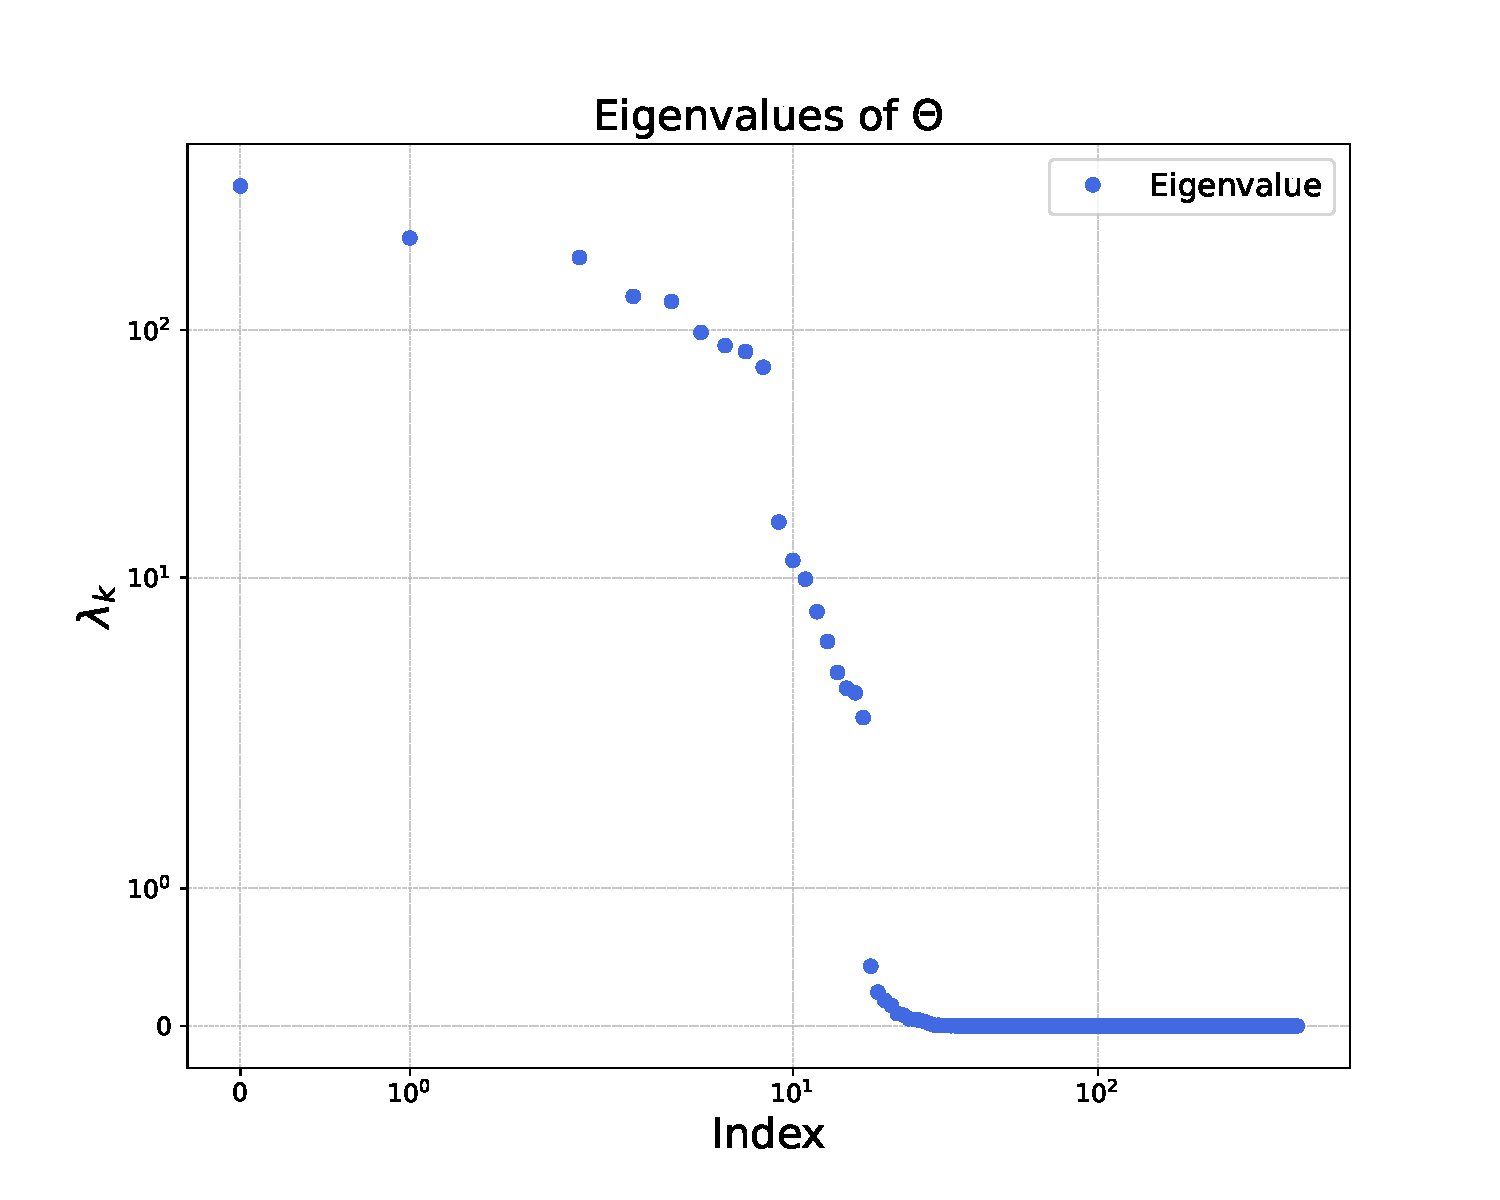
\includegraphics[width=0.48\textwidth]{ntk_eigvals.pdf}
  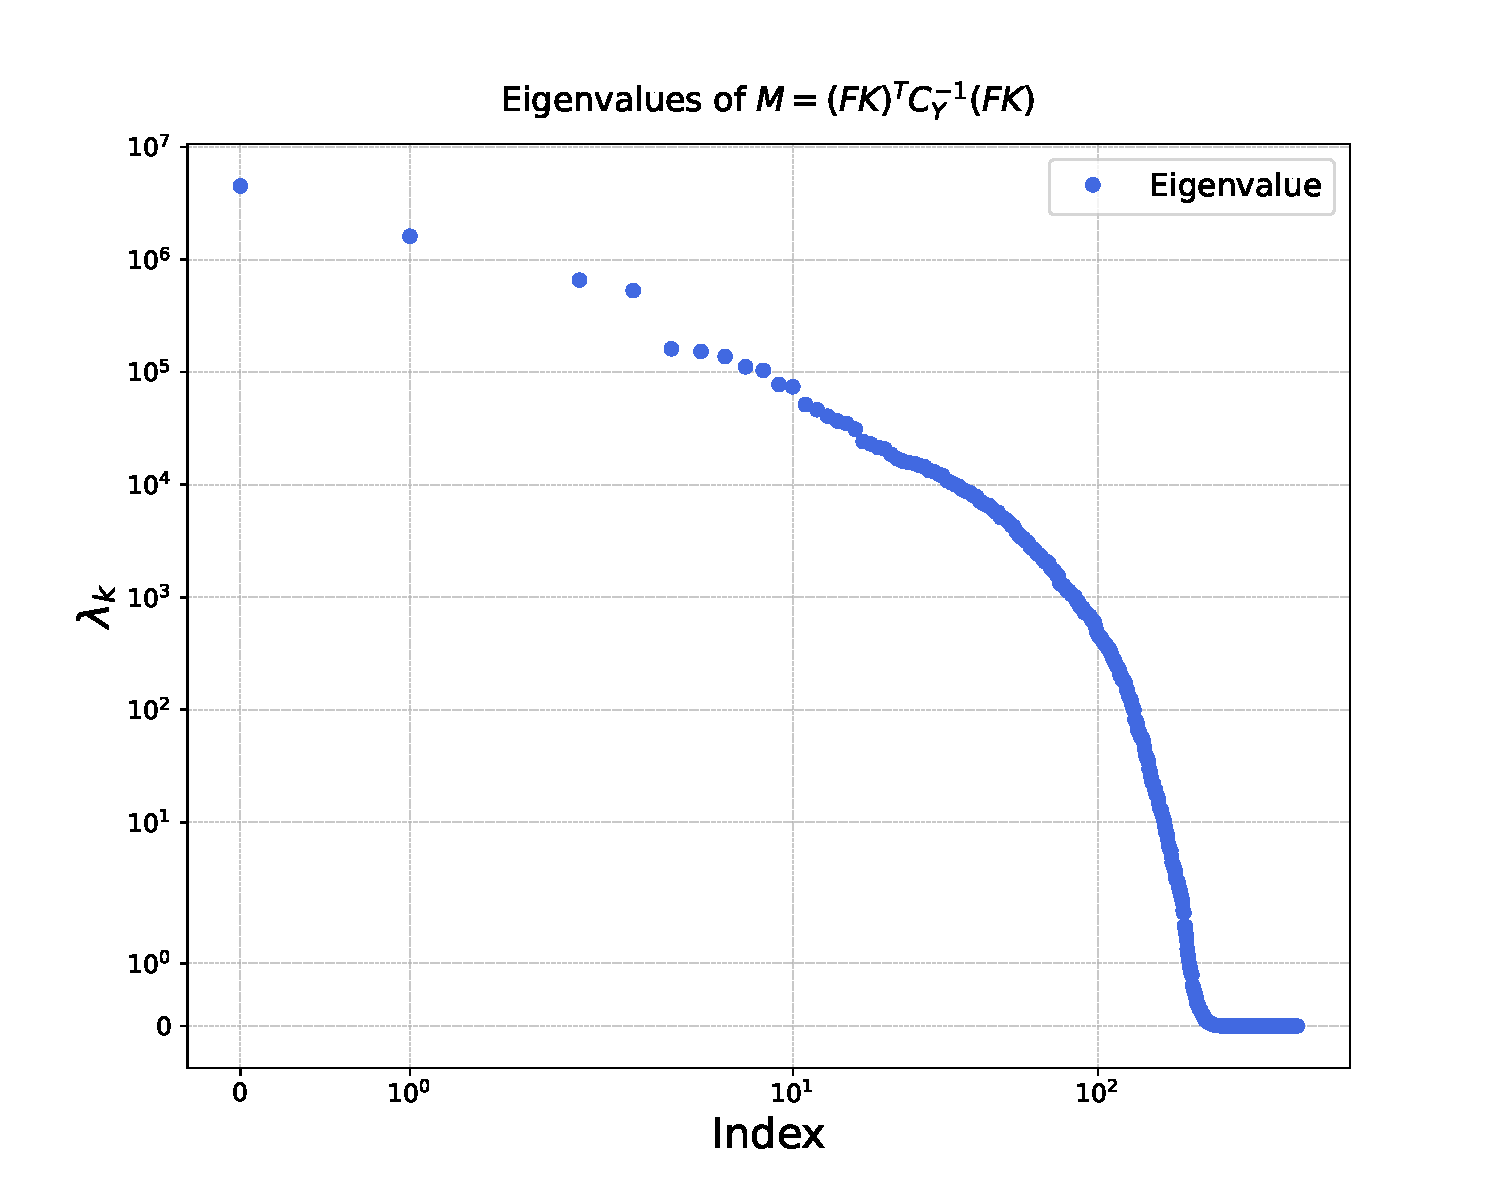
\includegraphics[width=0.48\textwidth]{m_eigvals.pdf}
  \caption{Eigenvalues of the NTK (left) and of the matrix $M$ (right) in 
    logarithmic scale.}
  \label{fig:NTKEigVals}
\end{figure}
%%%%%%%%%%%%%%%%%%%%%%%%%%
The eigenvalues of the NTK, together with those of the matrix $M$, are displayed in
Fig.~\ref{fig:NTKEigVals}. We rewrite the flow equation, Eq.~\ref{eq:FlowLinearDataNTK}, as
\begin{align}
    \label{eq:ft_b_ThetaMft}
    \frac{d}{dt} f_t = b - \Theta M f_t\, , 
\end{align}
where 
\begin{align}
    \label{eq:Defb}
    b = \Theta \FKtabT C_Y^{-1} y\, ,
\end{align}
while the matrix $M$ has been introduced above.  Using the eigendecomposition $M = R D R^T$, 
where $R$ is an orthogonal matrix, we introduce 
\begin{align}
    \label{eq:RotatedF}
    \tilde{f}_t = D^{1/2} R^T f_t\, , \quad \tilde{b} = D^{1/2} R^T b\, ,
\end{align}
so that 
\begin{align}
    \label{eq:EvolutionRotatedF}
    \frac{d}{dt} \tilde{f}_t &= \tilde{b} - D^{1/2} R^T \Theta R D^{1/2} \tilde{f}_t \\
        &= \tilde{b} - \tilde{H} \tilde{f}_t\, .
\end{align}
The solution, assuming that $\tilde{H}$ is independent of the flow time, is
\begin{align}
    \label{eq:FlowSolutionInFtilde}
    \tilde{f}_t = e^{-\tilde{H}t} \tilde{f}_0 + 
        \left(1 - e^{-\tilde{H}t}\right) \tilde{H}^{-1} \tilde{b}\, .
\end{align}
Taking the limit $t\to\infty$, we find
\begin{align}
    \label{eq:InfiniteTrainingF}
    f_\infty = M^{-1} \FKtabT C_Y^{-1} y = f^*\, .
\end{align}
This is consistent with the absolute minimum we found above. 
As before, in a L0 test, 
\begin{align}
    f_\infty = M^{-1} \FKtabT C_Y^{-1} \FKtab f^{\mathrm{in}} = f^{\mathrm{in}}\, .
\end{align}

\paragraph{Evolution for $\epsilon_t$.}
We can rewrite Eq.~\ref{eq:FlowLinearDataNTK} as 
\begin{align}
    \label{eq:FlowLinearDataNTKEpsilon}
    \frac{d}{dt} \epsilon_t &= - \FKtab \frac{d}{dt} f_t \nonumber \\
        &= - \FKtab \Theta \FKtabT C_Y^{-1} \epsilon_t \nonumber \\
        &= - \FKtab \Theta \FKtabT R_Y D_Y R_Y^T \epsilon_t\, ,
\end{align}
where we decompose $C_Y^{-1}=R_Y D_Y R_Y^T$.
Following the derivation for $f_t$, we define
\begin{align}
    \tilde{\epsilon}_t = D_Y^{1/2} R_Y^T \epsilon_t\, , 
\end{align}
one can readily check that 
\begin{align}
     \frac{d}{dt} \tilde{\epsilon}_t = 
        - \tilde{H}_\epsilon \tilde{\epsilon_t}\, ,
\end{align}
where 
\begin{align}
    \label{eq:HSymmetricDef}
    \tilde{H}_\epsilon  = D_Y^{1/2} R_Y^T \FKtab \Theta \FKtabT R_Y D_Y^{1/2}
\end{align}
is a symmetric, positive definite, matrix, and therefore
\begin{align}
    \label{eq:SolutionForEpsilon}
    \epsilon_t = R_Y D_Y^{-1/2} e^{-\tilde{H}_\epsilon t} D_Y^{1/2} R_Y^T \epsilon_0\, .
\end{align}
This result is consistent with the result above for the evolution of $f_t$. Now we need to 
check them numerically! 


\subsection*{Obsolete Material -- to be deleted, later}

We then project the flow equation for $f_t$, Eq.~\ref{eq:FlowLinearDataNTK}, in this basis
\begin{align}
    \label{eq:FlowEigenbasisNTK}
    \frac{d}{dt} f_{i,t} = b_i - \lambda_i M_{ij} f_{j,t}\, ,
\end{align} 
where
\begin{align}
    f_{i,t} &= (v_i, f_t)\, , \\
    b_i &= (v_i, \Theta \FKtabT C_Y^{-1} y)\, \\
    M_{ij} &= (v_i, \FKtabT C_Y^{-1} \FKtab v_j)\, .
\end{align}
Note that $M$ is symmetric and positive definite. We can write $M = R D^{1/2} D^{1/2} R^T$ and repeat the 
derivation we did for the $\epsilon$.

To be continued... 

At order $O(1)$ in an expansion in $1/n$, where $n$ is the width of the NN, $\Theta$ is constant during training, and the flow equation can be integrated analytically, 
\begin{align}
    \label{eq:IntegrateFlowAtLeadingOrder}
    f_t = M^{-1}\, \FKtabT\, \left[
        \left(1 - e^{-\hat{\Theta}_Yt}\right) y +
        e^{-\hat{\Theta}_Y t} \FKtab f_0
    \right]\, .
\end{align}
where 
\begin{align}
    \label{eq:DefineThetaM}
    \Theta_Y &= \FKtabT \Theta\, \FKtab\, , \\
    \hat{\Theta}_Y &= \Theta_Y C_Y^{-1}\, , \\    
    M &=  \FKtabT \FKtab\, .
\end{align}
Note that, if $\FKtab$ were invertible, then for $t\to\infty$
\begin{align}
    \FKtab f_\infty = \FKtab M^{-1} \FKtabT y = y\, ,
\end{align}
and the theoretical predictions go exactly through the points. However this is not true in the real life scenario where $\FKtab$ is {\em not}\ invertible. It is therefore interesting to compute the matrix (in data space)
\begin{align}
    \FKtab M^{-1} \FKtabT \, ,    
\end{align}
in order to understand how close the training can get to the training points. 

For points $f^*$ that do not enter in the computation of the theory prediction, the flow 
equation is
\begin{align}
    \label{eq:FlowStarLinearDataNTK}
    \frac{d}{dt} f^*_t = 
        \Theta^*_t\, \FKtab^T C_Y^{-1} \epsilon_t\, ,
\end{align}
where 
\begin{align}
    \label{eq:NTKStarDef}
    \Theta^*_t = \sum_{\mu,\nu}\, \lambda_{\mu\nu} \left(\nabla_\mu f^*_t\right)\, 
    \left(\nabla_\nu f_t\right)^T\, .
\end{align}
The solution to this flow equation is
\begin{align}
    \label{eq:IntegrateFlowAtLeadingOrderStar}
    f^*_t = \Theta^*\, \Theta^{-1}\, f_t \, . 
\end{align}
Need to check the constant term so that the boundary condition at $t=0$ is correct. 


\bibliographystyle{plain}
\bibliography{ntk.bib}

\appendix
\section{Null space of FK}
The FK tables can be regarded as a linear map from the space of PDFs to the space of 
data:
\begin{align}
  \FKtab : \mathbb{R}^{\PDF} \rightarrow \mathbb{R}^{\ndat} \,.
\end{align}
Note that the matrix corresponding to this linear map is not square, and hence $\FKtab 
\neq \FKtabT$. We can define the null space of the FK tables
\begin{equation}
  \ker \FKtab \equiv K_{\FKtab} = 
  \left\{
    f \in \mathbb{R}^{\PDF} \; : \; \FKtab \, f = 0
  \right\} \, ,
  \label{eq:ker_FK}
\end{equation}
together with its orthogonal space
\begin{equation}
  R_{\FKtab} \equiv K_{\FKtab}^{\bot} = 
  \left\{
    f \in \mathbb{R}^{\PDF} \; : \; f \cdot f_K = 0,
    \hspace{2mm} \forall f_K \in K_{\FKtab}
  \right\}\,.
\end{equation}
Note that 
\begin{align}
  \label{eq:KerFK->KerM}
  \FKtab f = 0 \Longrightarrow M f = 0\, .
\end{align}
The converse is also true, 
\begin{align}
  M f = 0 &\Longrightarrow (f, Mf) = 0 \\
    &\Longrightarrow (\FKtab f, C_Y^{-1} \FKtab f) = 0 \\
    &\Longrightarrow \FKtab f = 0\, ,
\end{align}
where the last inequality follows from the fact that $C_Y>0$.

For each of these two subspaces we can define a basis
\begin{align}
  & \B_{K} = \left\{ \pmb{u}^{(i)}_{K}\,, \hspace{2mm}  i=1,\dots, \dim K_{\FKtab} \right\} \,,\\
  & \B_{\bot} = \left\{ \pmb{u}^{(i)}_{\bot}\,, \hspace{2mm}  i=1,\dots, \dim R_{\FKtab} \right\} \,.
  \label{eq:FK_basis}
\end{align}
Remember that $K_{\FKtab} \bigoplus R_{\FKtab} = \mathbb{R}^{\PDF}$ and thus the basis $\B = \B_{K}
\bigoplus \B_{\bot}$ is a basis for $\mathbb{R}^{\PDF}$. Henceforth, when decomposing a vector in $\RPDF$, I 
will use the ordering $\left\{ \B_{K}, \B_{\bot} \right\}$. Hence, given $\pmb{f}\in \RPDF$, we can
write
\begin{equation}
  \pmb{f} = \pmb{f}_{K} + \pmb{f}_{\bot} 
          = \bpmat 
              f_K \\[2pt]
              f_{\bot}
            \epmat \,.
\end{equation}
Finally, note that $\FKtab$ is not symmetric (not even square). Thus, the right null space is not the same
as the left null space, in particular
\begin{align}
  \FKtab \pmb{u}_K = 0  \; \nRightarrow \; \pmb{u}_K^T \FKtab = 0 \,.
\end{align}

With the two bases in eqs.~\eqref{eq:FK_basis}, we can decompose the $\FKtab$ as follows
\begin{equation}
  \FKtab =
  \bpmat
    \FKtab_{KK}     & \FKtab_{K\bot} \\[3pt]
    \FKtab_{\bot K} & \FKtab_{\bot\bot}
  \epmat \,,
\end{equation}
where
\begin{align}
  \FKtab_{B_1 B_2} = \sum_{i=1}^{\dim\B_1} \sum_{j=1}^{\dim\B_2}
  \bra{u_{\B_1}^{(i)}} M \ket{u_{\B_2}^{(j)}} \;
  \pmb{u}_{\B_1}^{(i)} \pmb{u}_{\B_2}^{(j)}\,,
  \hspace{5mm}
  \B_1, \B_2 = K_{\FKtab}, R_{\FKtab}\,.
\end{align}
By definition of the kernel, we also have
\begin{align}
  \FKtab_{KK} = \FKtab_{\bot K} = 0 \,,
\end{align}
while $\FKtab_{K\bot}$ would be zero only if $\FKtab$ was diagonal. Thus, in the basis
$\B$, the FK tables can be expressed as
\begin{align}
  \FKtab =
  \bpmat
    0  & \FKtab_{K\bot} \\[3pt]
    0 & \FKtab_{\bot\bot}
  \epmat \,.
\end{align}
The product with a vector $\pmb{f} \in \RPDF$ becomes
\begin{equation}
  \FKtab \pmb{f} =
    \bpmat
      0  & \FKtab_{K\bot} \\[3pt]
      0  & \FKtab_{\bot\bot}
    \epmat
    \bpmat 
      f_K \\[2pt]
      f_{\bot}
    \epmat
    = \biggl(\FKtab_{K\bot} + \FKtab_{\bot\bot}\biggr) f_{\bot} \,.
\end{equation}

What are the implications for the matrix $M$? ...

\end{document}

%%% Local Variables:
%%% mode: latex
%%% TeX-master: t
%%% End:
